%%%%%%%% ICML 2018 EXAMPLE LATEX SUBMISSION FILE %%%%%%%%%%%%%%%%%
\documentclass{article}


% hyperref makes hyperlinks in the resulting PDF.
% If your build breaks (sometimes temporarily if a hyperlink spans a page)
% please comment out the following usepackage line and replace
% \usepackage{icml2018} with \usepackage[nohyperref]{icml2018} above.
\usepackage[draft]{hyperref}

% Attempt to make hyperref and algorithmic work together better:
\newcommand{\theHalgorithm}{\arabic{algorithm}}

% Use the following line for the initial blind version submitted for review:
\usepackage{icml2018}

% If accepted, instead use the following line for the camera-ready submission:
%\usepackage[accepted]{icml2018}

% The \icmltitle you define below is probably too long as a header.
% Therefore, a short form for the running title is supplied here:
\icmltitlerunning{CCP-IRL}

% HACK REMOVE
%\usepackage[showframe]{geometry}% http://ctan.org/pkg/geometry

\usepackage[utf8]{inputenc}
\usepackage{authblk}

\usepackage{icml2018}  %Required
\usepackage{times}  %Required
\usepackage{helvet}  %Required
\usepackage{courier}  %Required
\usepackage{url}  %Required
\usepackage{graphicx}  %Required
\usepackage{microtype}
\usepackage{subfigure}
\usepackage{booktabs} % for professional tables

\usepackage[T1]{fontenc}    % use 8-bit T1 fonts
\usepackage{amsfonts}       % blackboard math symbols
\usepackage{amsmath,amssymb}       % blackboard math symbols
\usepackage{nicefrac}       % compact symbols for 1/2, etc.
\usepackage{microtype}      % microtypography
\usepackage{bm}
\usepackage{algorithm}% http://ctan.org/pkg/algorithms
\usepackage{algorithmic}
%\usepackage{algpseudocode}% http://ctan.org/pkg/algorithmicx

%PDF Info Is Required:
\icmltitlerunning{CCP-IRL}

% \author[1]{Mohit Sharma}
% \author[1]{Kris M. Kitani}
% \affil[1]{Robotics Institute, Carnegie Mellon University}
% \affil[1]{\texttt{\{mohits1, kkitani\}@cs.cmu.edu}}
% \author[]{Joachim Groeger}
% %\affil[2]{Amazon.com}
% \affil[2]{\texttt{jrg@joachimgroeger.com}}


% \pdfinfo{
% /Title (Inverse Reinforcement Learning with Conditional Choice Probabilities)
% /Author (
%     Mohit Sharma, 
%     %\texttt{mohits1@andrew.cmu.edu}
%     %\and
%     Kris M. Kitani, 
%     %\texttt{kkitani@cs.cmu.edu}
%     %\and
%     Joachim Groeger
%     %\texttt{joachimgroeger@gmail.com})
% }

% === Kris' Macros === %
\usepackage{mathtools}
\usepackage{bm}
\renewcommand{\vec}[1]{\mbox{\bm{$#1$}}}
\def\argmax{\mathop{\rm arg\,max}}
\def\argmin{\mathop{\rm arg\,min}}

% === Mohit's Macros === %
\newcommand{\overbar}[1]{\mkern 1.5mu\overline{\mkern-1.5mu#1\mkern-1.5mu}\mkern 1.5mu}
\def\MSHangBox#1{%^
\begin{minipage}[t]{\textwidth}% Top-hanging minipage, will align on
			       % bottom of first line
\begin{tabbing} % tabbing so that minipage shrinks to fit
~\\[-\baselineskip] % Make first line zero-height
#1 % Include user's text
\end{tabbing}%^
\end{minipage}} % can't allow } onto next line, as {WIDEBOX}~x will not tie.

\usepackage{color}
\definecolor{purple}{rgb}{0.58,0,0.83}
\definecolor{red}{rgb}{1.0,0,0}
\definecolor{blue}{rgb}{0,1.0,0}
\definecolor{green}{rgb}{0,0,1.0}

\begin{document}

\twocolumn[
\icmltitle{Appendix for Inverse Reinforcement Learning with \\ Conditional Choice Probabilities}

% It is OKAY to include author information, even for blind
% submissions: the style file will automatically remove it for you
% unless you've provided the [accepted] option to the icml2018
% package.

% List of affiliations: The first argument should be a (short)
% identifier you will use later to specify author affiliations
% Academic affiliations should list Department, University, City, Region, Country
% Industry affiliations should list Company, City, Region, Country

% You can specify symbols, otherwise they are numbered in order.
% Ideally, you should not use this facility. Affiliations will be numbered
% in order of appearance and this is the preferred way.
\icmlsetsymbol{equal}{*}

\begin{icmlauthorlist}
\icmlauthor{Aeiau Zzzz}{equal,to}
\icmlauthor{Bauiu C.~Yyyy}{equal,to,goo}
\icmlauthor{Cieua Vvvvv}{goo}
\icmlauthor{Iaesut Saoeu}{ed}
\icmlauthor{Fiuea Rrrr}{to}
\icmlauthor{Tateu H.~Yasehe}{ed,to,goo}
\icmlauthor{Aaoeu Iasoh}{goo}
\icmlauthor{Buiui Eueu}{ed}
\icmlauthor{Aeuia Zzzz}{ed}
\icmlauthor{Bieea C.~Yyyy}{to,goo}
\icmlauthor{Teoau Xxxx}{ed}
\icmlauthor{Eee Pppp}{ed}
\end{icmlauthorlist}

\icmlaffiliation{to}{}
\icmlaffiliation{goo}{}
\icmlaffiliation{ed}{}

\icmlcorrespondingauthor{}{}
\icmlcorrespondingauthor{}{}

% You may provide any keywords that you
% find helpful for describing your paper; these are used to populate
% the "keywords" metadata in the PDF but will not be shown in the document
\icmlkeywords{Machine Learning, ICML}

\vskip 0.3in
]

% this must go after the closing bracket ] following \twocolumn[ ...

% This command actually creates the footnote in the first column
% listing the affiliations and the copyright notice.
% The command takes one argument, which is text to display at the start of the footnote.
% The \icmlEqualContribution command is standard text for equal contribution.
% Remove it (just {}) if you do not need this facility.

%\printAffiliationsAndNotice{}  % leave blank if no need to mention equal contribution
%\printAffiliationsAndNotice{\icmlEqualContribution} % otherwise use the standard text.

In this supplementary material we look at (1) the generalizability of CCP-IRL to non-parameteric reward estimation and (2) the robustness of CCP-IRL under noisy expert demonstrations.

\section{Non-Parametric Estimation of the Reward Function}

As discussed in the main paper, the CCP approach generalizes to both parameterized and non-parameterized reward functions. In the main paper we detail both the linear and non-linear formulations for parameterized reward functions. We now detail how the CCP approach can be used to estimate the reward function in a non-parameteric setting.  

To estimate the reward function non-parametrically we assume that shocks are TIEV and a normalization that one action generates a zero reward in every state. 
We now express the CCP in terms of choice specific value function differences. Define the choice specific value function for action $a$ as the reward from $a$ and the future value net of the payoff shock:
\begin{align}
\begin{split}
W_a(x_t) &= r_{}(x_t,a)+\beta  \cdot E_{x_{t+1}|a,x_t} \left[ \overline{V}(x_{t+1}) \right] 
\end{split}
\end{align}
The CCP expressed in terms of choice specific values is then:
\begin{align} 
\begin{split}
\sigma(a|x_t)&=\frac{\exp\left(r(x_t,a)+\beta E_{x_{t+1}|x_t,a} \overline{V}(x_{t+1})\right)}{\sum_{a'\in\mathcal{A}} \exp\left(r(x_t,a')+\beta E_{x_{t+1}|x_t,a'} \overline{V}(x_{t+1})\right)}\\
&=\frac{\exp(W_a(x_t))}{\sum_{a'\in\mathcal{A}} \exp(W_{a'}(x_t))}
\end{split}
\end{align}
Denote the action with zero reward by $a_0$. Multiply the CCP by $\frac{\exp(-W_{a_0}(x_t))}{\exp(-W_{a_0}(x_t))}$ which leads to  
\begin{align}
\begin{split}
\sigma(a|x_t)&=\frac{\exp(W_a(x_t)-W_{a_0}(x_t))}{\sum_{a'} \exp(W_{a'}(x_t)-W_{a_0}(x_t))}\\
&=\frac{\exp(\Delta_a(x_t))}{\sum_{a'} \exp(\Delta_{a'}(x_t))}
\end{split}
\end{align}
where $\Delta_{a'}(x_t)=W_{a'}(x_t)-W_{a_0}(x_t)$
It is clear from the above that choice-specific value function differences between action $a$ and some other action $a'$ are equal to:
\begin{align}\label{eq:ccp_ratio}
\begin{split}
\frac{\sigma(a'|x_t)}{\sigma(a_0|x_t)}&=
\left[
\frac
  {\exp(\Delta_{a'}(x_t))}
  {\sum_{a''} \exp(\Delta_{a''}(x_t))}
\right]
\left[\frac{\exp(\Delta_{a_0}(x_t))}{\sum_{a''} \exp(\Delta_{a''}(x_t))}\right]^{-1}\\
&=\exp(\Delta_{a'}(x_t))
\end{split}
\end{align}
where the last equality follows from the fact that $\exp(\Delta_{a_0})=\exp(W_{a_0}(x_t)-W_{a_0}(x_t))=\exp(0)=1$.
Now we consider the choice specific value function for the base action $a_0$. 
\begin{align}
\begin{split}
W_{a_0}(x_t) &= \beta  \cdot E_{x_{t+1}|a_0,x_t} \left[ \overline{V}(x_{t+1}) \right] 
\end{split}
\end{align}
Recall that:
\begin{align} 
\begin{split}
\overline{V}(x_t) &=\ln\bigg[\sum_{a\in\mathcal{A}} \exp\big(r(x_t,a)
\\&\qquad+\beta \cdot E_{x_{t+1}|a,x_t} \left[ \overline{V}(x_{t+1}) \right] \big)\bigg]  +\gamma,
\end{split}
\end{align}
which we can re-write in terms of choice specific value functions as:
\begin{align} 
\begin{split}
\overline{V}(x_t) &=\ln\left[\sum_{a\in\mathcal{A}} \exp\left(W_a(x_t) \right)\right]+\gamma,
\end{split}
\end{align}
We can then write the above in terms of choice specific value function differences by multiplying and dividing by $\exp(W_{a_0}(x_t))$ inside of the summation
\begin{align}
\begin{split}
\overline{V}(x_t) &=\ln\left[\sum_{a\in\mathcal{A}} \exp\left(W_a(x_t) \right)\right]+\gamma
\\&=\ln\left[\sum_{a\in\mathcal{A}} \exp(W_a(x_t))\exp(-W_{a_0}(x_t))\exp(W_{a_0}(x_t))\right]+\gamma
\\&=\ln\left[\exp(W_{a_0}(x_t))\sum_{a\in\mathcal{A}} \exp(W_a(x_t)-W_{a_0}(x_t))\right]+\gamma\\
&=W_{a_0}(x_t)+\ln\left[\sum_{a\in\mathcal{A}} \exp(W_a(x_t)-W_{a_0}(x_t))\right]+\gamma\\
&=W_{a_0}(x_t)+\ln\left[\sum_{a\in\mathcal{A}} \exp(\Delta_a(x_t))\right]+\gamma
\end{split}
\end{align}
% And therefore using the ratio of CCPs in 
% \begin{align} 
% \begin{split}
% \overline{V}(x_t) &=W_{a_0}(x_t)+\ln\left[\sum_{a\in\mathcal{A}} \exp(W_a(x_t)-W_{a_0}(x_t))\right]+\gamma\\
% &=W_{a_0}(x_t)+\ln\left[\sum_{a\in\mathcal{A}} \exp(W_a(x_t)-W_{a_0}(x_t))\right]+\gamma\\
% \end{split}
% \end{align}
Using the CCP ratio from (\ref{eq:ccp_ratio}), the above can be expressed as:
\begin{align} 
\begin{split}
\overline{V}(x_t) &=W_{a_0}(x_t)+\ln\left[\sum_{a\in\mathcal{A}} \exp(\Delta_a(x_t))\right]+\gamma\\
&=W_{a_0}(x_t)+\ln\left[\sum_{a\in\mathcal{A}} \frac{\sigma(a|x_t)}{\sigma(a_0|x_t)}\right]+\gamma\\
&=W_{a_0}(x_t)+\ln\left[1+\sum_{a\in\mathcal{A}\setminus a_0} \frac{\sigma(a|x_t)}{\sigma(a_0|x_t)}\right]+\gamma
\end{split}
\end{align}
the value function for the base action $a_0$ can then be expressed as:
\begin{align}
\begin{split}
W_{a_0}(x_t)&=
 \beta E_{x_{t+1}|x_t,a_0}
\Bigg[W_{a_0}(x_{t+1}) \\
&\left. +\ln\left[1+ \sum_{a'\in\mathcal{A}\setminus a_0}\frac{\sigma(a'|x_{t+1})}{\sigma(a_0|x_{t+1})}\right]+\gamma\right]
\end{split}
\end{align}
The only unknown in the above is $W_{a_0}$ which can be solved for using fixed point iteration or matrix inversion. The value function for every state can then be estimated as:
\begin{eqnarray}
W_a(x_t)=\ln(\sigma(a|x_t))-\ln(\sigma(a_0|x_t))+W_{a_0}(x_t).\label{eq:v_backout}
\end{eqnarray}
It is then possible to estimate the reward function directly:
\begin{align}
\begin{split}
r(a,x_t)
&=W_a(x_t)- \beta E_{x_{t+1}|x_t,a}\Bigg\{
W_{a_0}(x_{t+1})
\\ &\left.\qquad +
\ln
  \left(
    1 + \sum_{a'\in\mathcal{A}\setminus a_0}\frac{\sigma(a|x_{t+1})}{\sigma(a_0|x_{t+1})}
  \right)
\right\}.
\end{split}
\end{align}

% \newpage
% \begin{align} \label{eq:ccps}
% \begin{split}
% \sigma(a|x_t)=\frac{\exp\left(r(x_t,a)+\beta E_{x_{t+1}|x_t,a} \overline{V}(x_{t+1})\right)}{\sum_{a'\in\mathcal{A}} \exp\left(r(x_t,a')+\beta E_{x_{t+1}|x_t,a'} \overline{V}(x_{t+1})\right)}
% \end{split}
% \end{align}

% \begin{align} \label{eq:exante_inversion}
% \begin{split}
% \overline{\mathbf{V}} &=\left[I-\sum_{a}(\mathbf{S}(a) \lambda) *\left[ \beta \mathbf{T}(a)  \right]\right]^{-1} \\
% & \qquad \times \left[\sum_{a}\mathbf{S}(a) *\left[ \mathbf{R}_{\theta}(a)+\tilde{\bm{\epsilon}}(a)\right]\right]
% \end{split}
% \end{align}

% Same as:
% \begin{align} \label{eq:exante_inversion}
% \begin{split}
% \overline{\mathbf{V}} &=\left[I-\sum_{a}(\mathbf{S}(a) \lambda) *\left[ \beta \mathbf{T}(a)  \right]\right]^{-1} \\
% & \qquad \times\sum_{a}\mathbf{S}(a) *\left[ \mathbf{R}_{\theta}(a)\right]+\left[I-\sum_{a}(\mathbf{S}(a) \lambda) *\left[ \beta \mathbf{T}(a)  \right]\right]^{-1}\left[\sum_{a}\mathbf{S}(a) *\tilde{\bm{\epsilon}}(a)\right]
% \end{split}
% \end{align}

% \begin{align} \label{eq:ccps}
% \begin{split}
% \ln\sigma(a|x_t)-\ln \sigma(a'|x_t)=\left(r(x_t,a)+\beta E_{x_{t+1}|x_t,a} \overline{V}(x_{t+1})\right)-\left(r(x_t,a')+\beta E_{x_{t+1}|x_t,a'} \overline{V}(x_{t+1})\right)
% \end{split}
% \end{align}

% \bibliography{references}
% \bibliographystyle{icml2018}

\section{Highway: Evaluating Noisy Experts}

\begin{figure}[b!]
\centering
  \begin{tabular}{cc}
    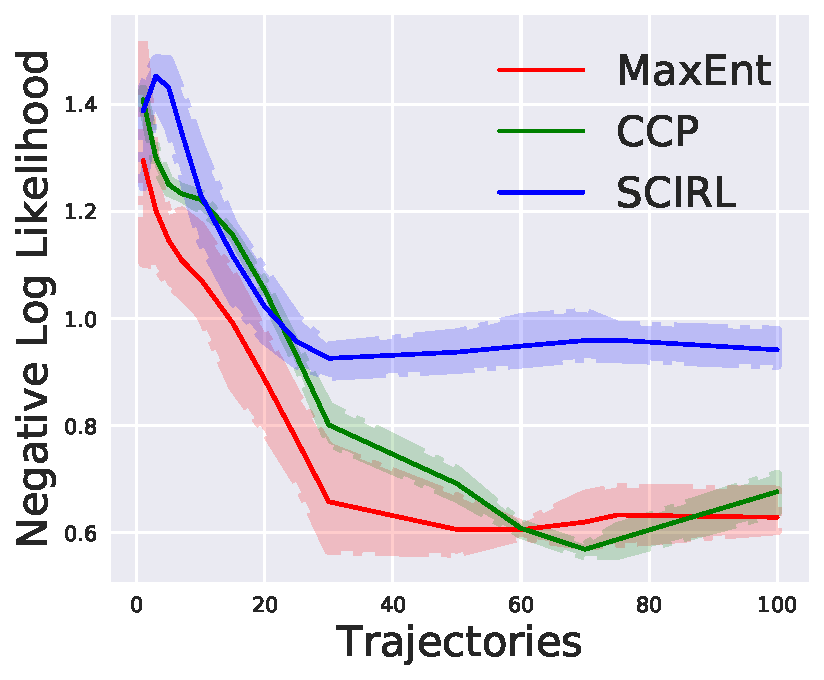
\includegraphics[width=0.22\textwidth]{images/highway/medium_mdp_noisy_expert/test_nll_algo_3.pdf}&
    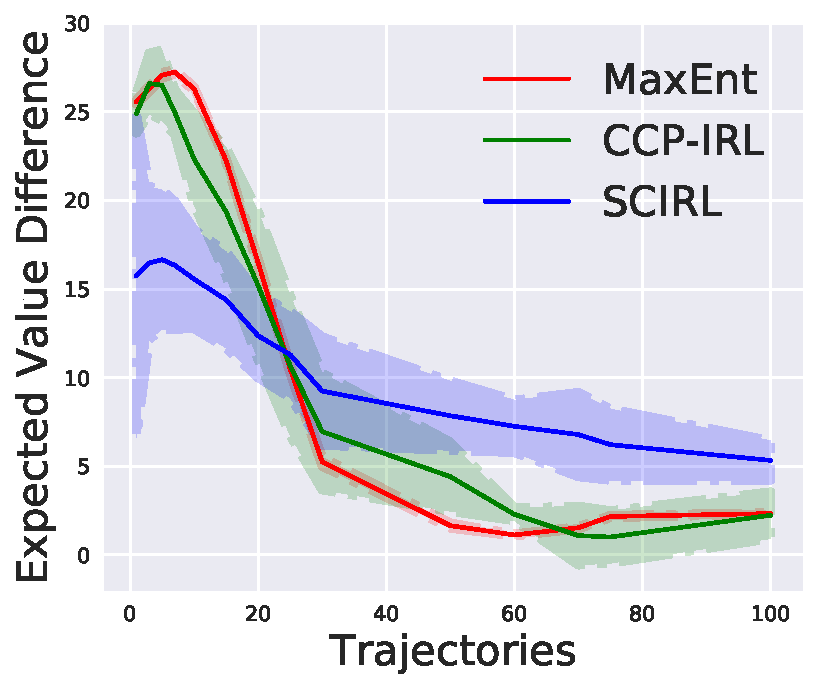
\includegraphics[width=0.22\textwidth]{images/highway/medium_mdp_noisy_expert/test_evd_algo_3.pdf}
    \end{tabular}
    \caption{Results for Highway MDP with 5,000 states with noisy expert demonstrations. These demonstrations were generated with noise probability $p=0.3$. Left: Minimum NLL results with varying number of trajectories. Right: Expected Value Difference results.}
    \label{fig:img_highway_noisy_exp}
\end{figure}

In this section, we illustrate the robustness of CCP-IRL against SCIRL when the expert demonstrations are noisy. Since, both CCP-IRL and MaxEnt-IRL use expert demonstrations to avoid solving the MDP problem, both of the algorithm's performance will be affected under noisy demonstrations. However, since SCIRL uses these noisy demonstrations direclty in a supervised learning framework we believe SCIRL's performance will be more adversely affected.

To simulate these noisy environments we use the Highway driving experiment as used in the main paper. However, instead of using learned expert demonstrations directly, we inject random noise into these demonstrations \emph{i.e.}, with a certain probability $p$ we end up taking a completely random action instead of the optimal action. We provide such noisy demonstrations to each of the IRL algorithms. 


\end{document}
